\chapter{Plug-in utilizzati}
	\section{Maven}
		Maven è stato utilizzato per gestire le varie dipendenze del progetto e la build automatica.
		Le dipendenze necessarie sono: 
		\begin{itemize}
			\item \emph{JUnit}: framework per lo unit-testing
			\item \emph{Guava}: libreria di GOOGLE che fornisce un hashmap bidirezionale
			\item \emph{Mockito}: framework utlizzato sempre per lo unit-testing
			\item \emph{Log4J}: framework per il logging 
		\end{itemize}
		
	\section{Travis}
		Travis viene utilizzato per la continuous integration. Il relativo file di configurazione è stato settato per utilizzare la jdk8 necessaria alla compilazione del progetto e per fornire il risultato della code coverage a coveralls.
		
	\section{Coveralls}
		Coveralls riceve i dati della coverage direttamente da Travis.
		
	\section{Docker}
		L'utilizzo principale di Docker è in realtà quello di usare docker compose per gestire il server di SonarQube senza doverlo effettivamente scaricare. 
		
	\section{Sonarqube}
		Sonarqube viene utilizzato tramite docker compose. E' stata scaricata l'ultima versione, attivando tutte le 395 regole disponibili per Java ad esclusione di quelle presenti in figura \ref{fig:sonarules}
		
		\begin{figure}
			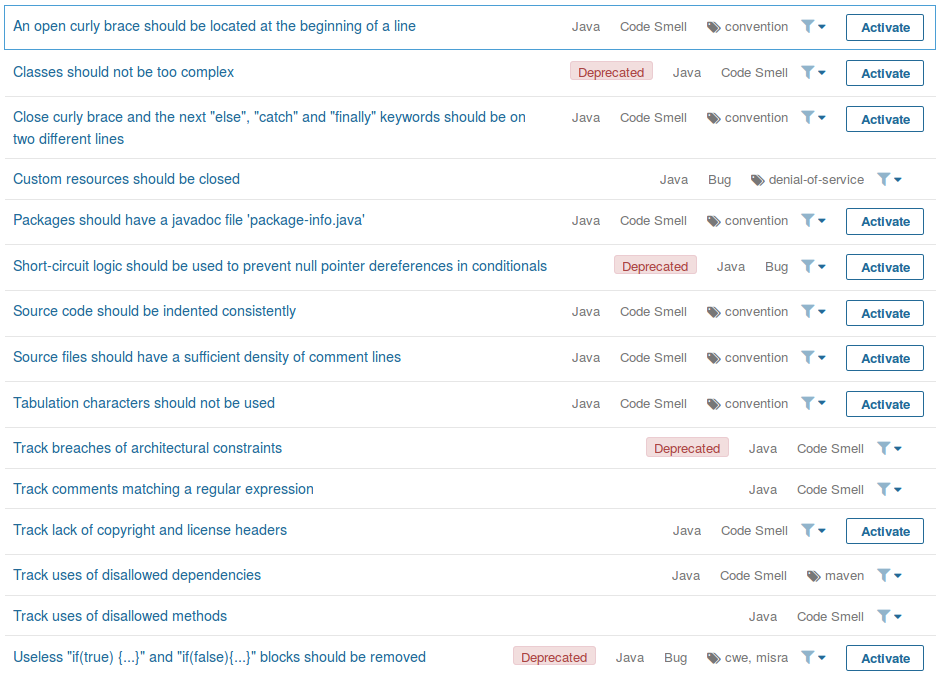
\includegraphics[scale=0.4]{img/sonarqube_rules}
			\caption{Regole disattivate}
			\label{fig:sonarules}
		\end{figure}
		
		Sono state escluse le regole deprecate, quelle riguardanti JavaDoc che non viene utilizzato in quanto questo progetto è pensato per un utilizzo personale e non per essere divulgato, quelle che contestano l'assenza delle informazioni di copyright e di licenza per lo stesso motivo e alcune regole ambigue di formattazione. Una di queste ad esempio è quella di mettere la parentesi graffa aperta di inizio blocco in una nuova linea che contrasta con quella che suggerisce di metterla sulla stessa riga.
		
		Il risultato della scansione utilizzando questi parametri è illustrato in figura \ref{fig:sonaresult}
		
		\begin{figure}
			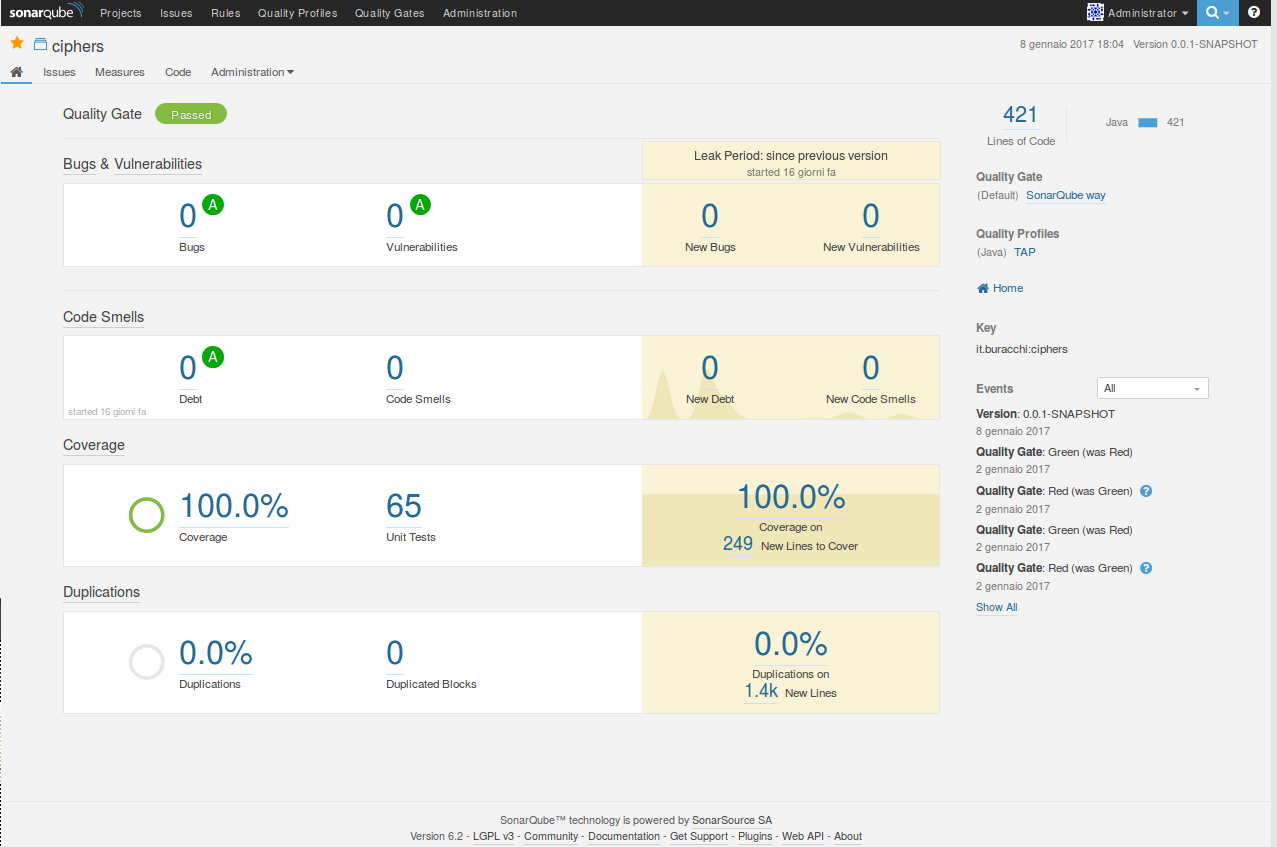
\includegraphics[scale=0.3]{img/sonaresult}
			\caption{Risultato della scansione}
			\label{fig:sonaresult}
		\end{figure}